\NeedsTeXFormat{LaTeX2e}
\documentclass[12pt, a4paper]{book}

\usepackage[utf8]{inputenc}
\setlength{\emergencystretch}{1em}
\usepackage[dvipsnames]{xcolor} 
\definecolor{halfgray}{gray}{0.55} % chapter numbers will be semi transparent .5 .55 .6 .0
\usepackage{xspace}
\usepackage{mparhack}
\let\oldmarginpar\marginpar
\renewcommand{\marginpar}[1]{\oldmarginpar%
 [\raggedleft\hspace{0pt}{#1}]%
 {\raggedright\hspace{0pt}{#1}}}

\usepackage{textcase} 
\usepackage{soul} % for letterspacing 
                \sodef\allcapsspacing{\upshape}{0.15em}{0.65em}{0.6em}%
                \sodef\lowsmallcapsspacing{\scshape}{0.075em}{0.5em}{0.6em}%   
                \DeclareRobustCommand{\spacedallcaps}[1]{\MakeTextUppercase{\allcapsspacing{#1}}}%   
                \DeclareRobustCommand{\spacedlowsmallcaps}[1]{\MakeTextLowercase{\textsc{\lowsmallcapsspacing{#1}}}}%\protect
                
 \DeclareRobustCommand{\spacedallcaps}[1]{\MakeTextUppercase{\allcapsspacing{#1}}}
 
% \newfont{\chapterNumber}{eurb10 scaled 7000}
\newfont{\chapterNumber}{pplr9d scaled 7000}
 
\usepackage{titlesec}
% something like Bringhurst  
    \titleformat{\chapter}[display]%
        {\relax} % format
{\mbox{}\oldmarginpar{\vspace*{-3\baselineskip}\color{halfgray}\chapterNumber\thechapter}} % label
{0pt} % sep
{\raggedright\spacedallcaps} % before-code
[\normalsize\vspace*{.8\baselineskip}\titlerule] % after-code 
    
    % sections \FloatBarrier
    \titleformat{\section}
        {\relax}{\textsc{\MakeTextLowercase{\thesection}}}{1em}{\spacedlowsmallcaps}
    % subsections
    \titleformat{\subsection}
        {\relax}{\textsc{\MakeTextLowercase{\thesubsection}}}{1em}{\normalsize\itshape}
    % subsubsections
    \titleformat{\subsubsection}
        {\relax}{\textsc{\MakeTextLowercase{\thesubsubsection}}}{1em}{\normalsize\itshape}
        
\usepackage[titles]{tocloft}

\renewcommand{\cftdot}{} %empty {} for no dots. you can have any symbol inside.

% chapters
        	\renewcommand{\cftchappresnum}{\scshape\MakeTextLowercase}%
            \renewcommand{\cftchapfont}{\scshape}%
            \renewcommand{\cftchappagefont}{\normalfont}%
            
            \renewcommand{\cftsecpresnum}{\scshape\MakeTextLowercase}%
    	\renewcommand{\cftsecfont}{\normalfont}%
      \renewcommand{\cftsecpagefont}{\normalfont}%
      
%      \renewcommand{\cftchapleader}{\hspace{1.5em}}% 
%            	\renewcommand{\cftchapafterpnum}{\cftparfillskip}% 
%            	\renewcommand{\cftsecleader}{\hspace{1.5em}}% 
%      	\renewcommand{\cftsecafterpnum}{\cftparfillskip}%
%      	\renewcommand{\cftsubsecleader}{\hspace{1.5em}}% 
%      	\renewcommand{\cftsubsecafterpnum}{\cftparfillskip}

	\usepackage[automark]{scrpage2} % provides headers and footers (KOMA Script)
    \clearscrheadings
    \setheadsepline{0pt}
    \renewcommand{\chaptermark}[1]{\markboth{\spacedlowsmallcaps{#1}}{\spacedlowsmallcaps{#1}}}
    \renewcommand{\sectionmark}[1]{\markright{\thesection\enspace\spacedlowsmallcaps{#1}}} 
    \lehead{\mbox{\llap{\small\thepage\kern2em}\headmark\hfil}}
    \rohead{\mbox{\hfil{\headmark}\rlap{\small\kern2em\thepage}}}
    \renewcommand{\headfont}{\small}  



\usepackage[osf, sc]{mathpazo}
\linespread{1.05}
\usepackage{blindtext}
\usepackage{tikz}
\usetikzlibrary{shapes, arrows,calc,patterns,decorations.pathmorphing, decorations.markings}
\usepackage{tikz-3dplot}
\usepackage{tikzscale}
\usepackage{epsfig}
\usepackage{epstopdf}
\usepackage{graphicx}
\usepackage{caption}
\usepackage{subcaption}
\usepackage{keyval}
\usepackage{float}
\usepackage{listings}
\usepackage{color}
\usepackage{textcomp}
\usepackage{datetime}
\usepackage[numbers, sort&compress, comma]{natbib}
\usepackage{subeqnarray}
\usepackage{longtable}
\usepackage{booktabs}
\usepackage{array}
\usepackage{bm}
\usepackage{amsmath}
\usepackage{amsfonts}
\usepackage{amssymb}
\usepackage{mathtools}
\usepackage{units}
\usepackage{pgfplots}
\usetikzlibrary{external}
\tikzexternalize[prefix=Tikz/]
\tikzsetexternalprefix{Figures/}
\pgfplotsset{
    tick label style={font=\scriptsize},
    label style={font=\small},
	title style={font=\normalsize\normalfont},
    legend style={font=\scriptsize}
}
% \tikzset{external/force remake} % Remake all tikz pictures.
\usepackage{listings}

\definecolor{mygreen}{rgb}{0,0.6,0}
\definecolor{myviolette}{rgb}{160,32,240}

\usepackage [linktocpage=all]{hyperref}
\hypersetup{
  pdftitle    = {Titel},
  pdfsubject  = {Electrical Engineering},
  pdfauthor   = {Robin Weiß},
  pdfkeywords = {Bachelor Thesis} ,
  pdfcreator  = {pdflatex},
  pdfproducer = {LaTeX}
}

\usepackage[acronym, nopostdot, nonumberlist, ucmark=true]{glossaries}
\newglossary[nlg]{notation}{not}{ntn}{Notation}

\setcounter{tocdepth}{2}
\setcounter{secnumdepth}{2}

\clubpenalty = 10000
\widowpenalty = 10000 
\displaywidowpenalty = 10000

\newcommand{\clearemptydoublepage}
{\newpage{\pagestyle{empty}\cleardoublepage}}

\makeglossaries
\setlength{\glsdescwidth}{0.8\linewidth}


\newacronym{CITIC-UGR}{CITIC-UGR}{Research Centre for Information and Communications Technologies of the University of Granada}

\newacronym{IMUs}{IMUs}{inertial measurement units}

\newacronym{MIMUs}{MIMUs}{magnetic inertial measurement units}
\newglossaryentry{not:F}{
  type=notation,
  name={$\mathbf{f}$},
  description={Force vector, $\mathbf{f} \in \mathbb{R}^3$},
  sort={f}}
  
\newglossaryentry{not:B_v}{
  type=notation,
  name={$\mathbf{B}$},
  description={Control matrix that relates the control input to the state $\mathbf{x}$},
  sort={Ba}}
 
\newglossaryentry{not:m}{
  type=notation,
  name={$m$},
  description={Mass},
  sort={m}}
  
\newglossaryentry{not:sigma}{
  type=notation,
  name={$\sigma$},
  description={Standard deviation},
  sort={sigma}}
  
\newglossaryentry{not:sigma_2}{
  type=notation,
  name={$\sigma^2$},
  description={Variance},
  sort={sigma}}
  
\newglossaryentry{not:mu}{
  type=notation,
  name={$\mu$},
  description={Mean value of conditional probability density},
  sort={sigma}}
  
\newglossaryentry{not:n}{
  type=notation,
  name={$n$},
  description={Fixed discrete time, non-dimensional number, or number of iterations, applied to recursive algorithms},
  sort={n}}
  
\newglossaryentry{not:a}{
  type=notation,
  name={$\mathbf{a}$},
  description={Acceleration vector, $\mathbf{a} \in \mathbb{R}^3$},
  sort={a}}
  
\newglossaryentry{not:impulse}{
  type=notation,
  name={$h_0, h_1, h_2, \dots$},
  description={Impulse response of a linear discrete-time filter},
  sort={h}}
  
\newglossaryentry{not:input}{
  type=notation,
  name={$z(0), z(1), z(2), \dots$},
  description={Time series that serves as input to a linear discrete-time filter},
  sort={yaa}}
  
\newglossaryentry{not:desired_response}{
  type=notation,
  name={$d$},
  description={Desired filter response of a linear discrete-time filter},
  sort={d}}
  
\newglossaryentry{not:error_signal}{
  type=notation,
  name={$e$},
  description={Error signal of a linear discrete-time filter},
  sort={e}}
  
\newglossaryentry{not:t}{
  type=notation,
  name={$t$},
  description={Continuous time},
  sort={t}}

\newglossaryentry{not:x_v}{
  type=notation,
  name={$\mathbf{x}$},
  description={State vector of a linear dynamical system},
  sort={xb}}
  
\newglossaryentry{not:x}{
  type=notation,
  name={$x$},
  description={One-dimensional location},
  sort={x}}
  
\newglossaryentry{not:displacement}{
  type=notation,
  name={$\Delta x$},
  description={One-dimensional displacement in $x$-direction},
  sort={x}}
  
\newglossaryentry{not:x_hat}{
  type=notation,
  name={$\hat{x}$},
  description={Estimate of $x$},
  sort={xa}}
  
\newglossaryentry{not:w_v}{
  type=notation,
  name={$\mathbf{w}$},
  description={Process noise vector},
  sort={wa}}
  
\newglossaryentry{not:v}{
  type=notation,
  name={$\mathbf{v}$},
  description={Measurement noise vector},
  sort={v}}
  
\newglossaryentry{not:u}{
  type=notation,
  name={$u$},
  description={Nominal velocity},
  sort={u}}
  
\newglossaryentry{not:w}{
  type=notation,
  name={$w$},
  description={Noise term},
  sort={w}}

\newglossaryentry{not:x_hat_v}{
  type=notation,
  name={$\hat{\mathbf{x}}$},
  description={Estimate of the state vector of a linear dynamical system},
  sort={xd}}
  
\newglossaryentry{not:x_hat_minus}{
  type=notation,
  name={$\hat{\mathbf{x}}^-_k$},
  description={A priori estimate of $\hat{\mathbf{x}}$, conditioned on all prior measurements except the one at time $t_k$},
  sort={xe}}
  
\newglossaryentry{not:z}{
  type=notation,
  name={$\mathbf{z}$},
  description={Observation or measurement vector of a dynamical system},
  sort={zaa}}
  
\newglossaryentry{not:H}{
  type=notation,
  name={$\mathbf{H}$},
  description={Measurement sensitivity matrix defining the linear relationship between the state of the dynamical system and the measurements that can be made},
  sort={Ha}}
  
\newglossaryentry{not:K_v}{
  type=notation,
  name={$\mathbf{K}$},
  description={Kalman gain matrix},
  sort={Kaa}}
  
\newglossaryentry{not:K}{
  type=notation,
  name={$K$},
  description={Weighting factor},
  sort={Ka}}
  
 \newglossaryentry{not:k}{
  type=notation,
  name={$k$},
  description={Discrete time normalised to sampling interval, that is sample number, $k \in \mathbb{N}^0$},
  sort={k}}
  
\newglossaryentry{not:P}{
  type=notation,
  name={$\mathbf{P}$},
  description={Covariance matrix of state estimation uncertainty},
  sort={P}}
  
\newglossaryentry{not:Q}{
  type=notation,
  name={$\mathbf{Q}$},
  description={Covariance matrix of process noise in the system state dynamics},
  sort={Q}}
  
\newglossaryentry{not:R}{
  type=notation,
  name={$\mathbf{R}$},
  description={Covariance matrix of observational (measurement) uncertainty},
  sort={R}}
  
\newglossaryentry{not:phi}{
  type=notation,
  name={$\bm{\Phi}$},
  description={State transition matrix of a discrete linear dynamical system},
  sort={phiaa}}
  
\newglossaryentry{not:x_k}{
  type=notation,
  name={$\mathbf{x}_k$},
  description={The $k$th element of a sequence $\dots$, $\mathbf{x}_{k-1}$, $\mathbf{x}_k$, $\mathbf{x}_{k+1}, \dots$ of vectors},
  sort={xc}}
  
 \newglossaryentry{not:unit-delay}{
  type=notation,
  name={$z^{-1}$},
  description={Unit-delay},
  sort={za}}
  
\newglossaryentry{not:roll}{
  type=notation,
  name={$\phi$},
  description={Roll angle that determines the rotation around the $x$-axis},
  sort={phi}}
  
\newglossaryentry{not:pitch}{
  type=notation,
  name={$\theta$},
  description={Pitch angle that determines the rotation around the $y$-axis},
  sort={theta}}
  
\newglossaryentry{not:yaw}{
  type=notation,
  name={$\psi$},
  description={Yaw angle that determines the rotation around the $z$-axis},
  sort={psi}}

\newglossaryentry{not:navigation_frame}{
  type=notation,
  name={$x, y, z$},
  description={Axes of the fixed world frame},
  sort={xayaza}}
  
\newglossaryentry{not:body_frame}{
  type=notation,
  name={$X, Y, Z$},
  description={Axes of the moving body frame},
  sort={xayazb}}
  
\newglossaryentry{not:transformation_matrix}{
  type=notation,
  name={$\mathbf{T}$},
  description={Transformation matrix},
  sort={Ta}}
  
\newglossaryentry{not:transformation_matrix_bn}{
  type=notation,
  name={$\mathbf{C}_{bw}$},
  description={Transformation matrix transforming a position vector from the body frame to the world frame},
  sort={Cbn}}
  
\newglossaryentry{not:transformation_matrix_nb}{
  type=notation,
  name={$\mathbf{C}_{wb}$},
  description={Transformation matrix transforming a position vector from the world frame to the body frame},
  sort={Cnb}}
  
\newglossaryentry{not:omega}{
  type=notation,
  name={$\bm{\Omega}_{\mathbf{E} \rightarrow \mathbf{E}'}$},
  description={Function that transforms a position vector $\mathbf{p}$ in the vector space $\mathbf{E}$ into the vector $\mathbf{p}^{'}$ in the vector space $\mathbf{E}^{'}$},
  sort={Om}}
  
\newglossaryentry{not:position_vector}{
  type=notation,
  name={$\mathbf{p}$},
  description={Position vector in a three-dimensional vector space},
  sort={p}}
  
\newglossaryentry{not:phi_vec}{
  type=notation,
  name={$\bm{\phi}$},
  description={Functional denoting the \emph{non-linear} transition matrix function of a discrete dynamical system},
  sort={phia}}
  
\newglossaryentry{not:h_vec}{
  type=notation,
  name={$\mathbf{h}$},
  description={Functional denoting the \emph{non-linear} measurement matrix function of a discrete dynamical system},
  sort={h}}

\newglossaryentry{not:resonance_freq}{
  type=notation,
  name={$\Omega$},
  description={Resonance frequency},
  sort={Omega}}
  
\newglossaryentry{not:force_one_d}{
  type=notation,
  name={$F$},
  description={One-dimensional force},
  sort={f}}
  
\newglossaryentry{not:damping_c}{
  type=notation,
  name={$D$},
  description={Damping coefficient},
  sort={D}}
  
\newglossaryentry{not:amplitude}{
  type=notation,
  name={$a$},
  description={Amplitude of an oscillating mode},
  sort={a}}
  
\newglossaryentry{not:angular_v_scalar}{
  type=notation,
  name={$\omega$},
  description={Scalar angular velocity},
  sort={omega}}
  
\newglossaryentry{not:spring_constant}{
  type=notation,
  name={$k_x$},
  description={Spring constant along the $x$-axis},
  sort={kx}}
  
\newglossaryentry{not:gravity}{
  type=notation,
  name={$\mathbf{g}$},
  description={Gravity vector},
  sort={g}}
  
\newglossaryentry{not:angular_velocity}{
  type=notation,
  name={$\bm{\omega}$},
  description={Angular velocity, $\bm{\omega} \in \mathbb{R}^3$},
  sort={omega}}

\newglossaryentry{not:mass_velocity}{
  type=notation,
  name={$\mathbf{v}$},
  description={Mass velocity, $\mathbf{v} \in \mathbb{R}^3$},
  sort={va}}  
  
\newglossaryentry{not:orthonormal_basis}{
  type=notation,
  name={$\mathbf{E}$},
  description={Orthonormal basis $\{x, y, z\} \in \mathbb{R}^3$},
  sort={E}}  
  
\newglossaryentry{not:identity_matrix}{
  type=notation,
  name={$\mathbf{I}_n$},
  description={Identity matrix $\mathbf{I}_n \in \mathbb{R}^n$},
  sort={I}}  

\newglossaryentry{not:magnitude_gravity}{
  type=notation,
  name={$\|\mathbf{g}\|$},
  description={Magnitude of the gravity vector},
  sort={ga}}    
  
\newglossaryentry{not:sampling interval}{
  type=notation,
  name={$T_s$},
  description={Sampling period},
  sort={T}}    
  
    

% Add all glossary entries not only the referenced ones.
\glsaddall
    

\begin{document}

	\frontmatter
	
	\pagestyle{scrheadings}

	\begin{titlepage}
\label{ch:titlepage}

\begin{center}


\includegraphics[width=7cm]{images/universidad_de_granada.eps}
	\hfill

\includegraphics[width=5cm]{images/fh-muenster.eps} 

\vspace{2.5cm}

{\large \textsc{Münster University of Applied Sciences}}

Department of Electrical Engineering and Computer Science

\vspace{1.5cm}

{\large Bachelor Thesis}

\vspace{0.8cm}

\begin{LARGE}
\textsc{kalman filtering applied to orientation estimation in gait analysis}
\end{LARGE}

\vspace{1.8cm}

\begin{minipage}{0.4\textwidth}
\begin{flushleft}
\emph{Author:} \\
Robin Weiß
\end{flushleft}
\end{minipage}
\hfill
\begin{minipage}{0.5\textwidth}
\begin{flushright}
\emph{Supervisors:} \\
Prof. Dr.-Ing. Peter Glösekötter \\
Ph.D. Alberto Olivares Vicente \\
Prof. Dr. med. Kai Bötzel
\end{flushright}
\end{minipage}

\vspace{2.0cm}
	
\textit{A thesis submitted in partial fulfilment of the requirements for the degree\\
of Bachelor of Science in Electrical Engineering}

\vfill

\monthname \: \the\year 

\end{center}

\end{titlepage}

	\clearemptydoublepage
	
	\setcounter{page}{1}	
	\phantomsection
	\addcontentsline{toc}{chapter}{Statement of Authorship}
	\thispagestyle{empty}

\subsection*{Statement of Authorship}
I hereby certify that this bachelor thesis has been composed by myself, and describes my own work, unless otherwise acknowledged in the text. All references and verbatim extracts have been quoted, and all sources of information have been specifically acknowledged. It has not been accepted in any previous application for a degree.

\vspace{1cm}

\noindent 
Granada, $\the\day^{\text{th}}$ \monthname \: \the\year

\vspace{2cm}

\noindent
Robin Weiß

	\clearemptydoublepage
	
	\chapter*{Preface}

This thesis entitled ``Analysis of anticipatory postural adjustments of Parkinson's patients using inertial sensors'' was submitted in partial fulfillment of the requirements for the degree of Bachelor of Science in Electrical Engineering awarded from the Münster University of Applied Sciences.

I took part in a conjoint project between the Research Centre for Information and Communications Technologies of the University of Granada (CITIC-UGR)\nomenclature{CITIC-UGR}{Research Centre for Information and Communications Technologies of the University of Granada} and the Department of Neurology of the Klinikum Großhadern in Munich, which is part of the Ludwig-Maximilians University. The objective of this thesis was to carry out an analysis of the so called anticipatory postural adjustments, which are the movements by a human subject between the moment he initiates gait and the first step.
	\clearemptydoublepage

	

\subsection*{Abstract}

This thesis entitled ``Analysis of anticipatory postural adjustments of Parkinson's patients using inertial sensors'' was submitted in partial fulfilment of the requirements for the degree of Bachelor of Science in Electrical Engineering. 

I took part in a conjoint project between the Research Centre for Information and Communications Technologies of the University of Granada (CITIC-UGR) and the Department of Neurology of the Klinikum Großhadern in Munich, which is part of the Ludwig-Maximilians University. The objective of this thesis was to carry out an analysis of the so called anticipatory postural adjustments, which are the movements by a human subject between the moment he initiates gait and the first step.

	\clearemptydoublepage
	
	\phantomsection
	\addcontentsline{toc}{chapter}{Contents}
	\tableofcontents
	\clearemptydoublepage
		
	\listoffigures
	\addcontentsline{toc}{chapter}{List of Figures}
	\clearemptydoublepage

%	\listoftables
%	\addcontentsline{toc}{chapter}{List of Tables}
%	\clearemptydoublepage	
	
	\printglossary[type=acronym, title={Abbreviations}, style=super]
	\addcontentsline{toc}{chapter}{Abbreviations}
	\clearemptydoublepage
    
    \printglossary[type=notation, style=super]
    \addcontentsline{toc}{chapter}{Notation}
    \clearemptydoublepage
	
	\mainmatter
		
	\chapter{Introduction}
\label{ch:Introduction}

Monitoring and assessment of human body motion, in particular the analysis of gait, has become an integral part of medical diagnosis, therapy techniques, and rehabilitation \cite{tao_gait_2012}. \emph{Gait analysis} involves the measurement and assessment of quantitative parameters that characterise human locomotion. First research in this field was conducted in the late 19\textsuperscript{th} century \cite{tao_gait_2012}. The quantitative data enable physicians to diagnose a variety of medical conditions, validate treatment success, set goals in rehabilitation and regularly alter them when necessary. However, standard gait analysis based on multi-camera motion capture systems and force platforms require specialised gait laboratories, expensive equipment, and lengthy setup times. Moreover, the assessments of gait based on measurements performed in clinical settings might not be truly representative \cite{bonato_advances_2005}.

Unobtrusive wearable sensors mitigate the aforementioned limitations. Low cost sensors have been employed in clinical and home environments to constantly monitor the movements of patients \cite{godfrey_direct_2008}. The progressive miniaturisation of inertial and magnetic field sensors has made them more acceptable to patients and has consequently lead to an increasingly pervasive adoption for medical applications \cite{wee_soon_ambulatory_2008}, especially in the truly representative home environment.  Among others, wearable inertial and magnetic sensors are used to assess \emph{gait kinematics}. An extensive description is presented in Section \ref{sec:MARG_sensors_medical}. \emph{Kinematics} is a branch of classical mechanics, which is concerned with motion of objects without reference to the forces causing the motion. Position, velocity and acceleration are of particular interest in kinematics.

Determining the position of the legs is essential in gait analysis. The position, i.\,e. the orientation, can be estimated from inertial data. For the application in health care accurate orientation estimates are crucial. A high degree of precision based on data from miniaturised sensors necessitates adequate signal processing, in order to mitigate the influence of disruptive factors, such as bias instability and noise, among others. The signal processing of inertial and magnetic data encompasses calibration, adaptive filtering, and sensor fusion. The latter two are a part of this work.

\section{Motivation}

Gait analysis provides a powerful means to derive diagnostic information about the functioning of the musculoskeletal, vestibular, and central and peripheral nervous system \cite{bennett_extended_2013}. Accurate orientation estimation of the extremities by means of wearable inertial and magnetic field sensors allows objective assessment of human gait and can therefore benefit medical applications without the aforementioned constraints of camera based motion capture systems. A more reliable and more precise orientation estimation would enable an even more informative gait analysis. A multitude of applications in the medical field would profit from such an enhanced gait analysis \cite{wong_clinical_2007}. The direct relation to health care and the resulting possibility to improve the quality of life of many patients was the motivation for this thesis.

\section{Goals}

The goal of this thesis was implementing a new Kalman filter based orientation algorithm proposed by \citeauthor{bennett_motion_2014} in \cite{bennett_motion_2014}. Thus the estimation of orientation angles of the human leg by means of inertial and magnetic sensors should be improved. The filter algorithm should be implemented using \textsc{Matlab}\textsuperscript{\textregistered} and validated against existing algorithms by comparing their respective \gls{RMSE}. An existing system for human body motion analysis based on wearable sensors was available, so that no new hardware had to be developed to gather the movement data. A detailed description of the so-called GaitWatch system is found at the end of Chapter \ref{ch:MARG}.

\section{Methodology}

This document presents my work within the overall project in a chronological order. Subsequent to the previous introductory overview of the topic and the definition of the project objectives, this chapter ends with a description of the state of the art. To accomplish the tasks defined in the previous section, I had to acquire knowledge regarding various subjects. Chapters 2 to 4 outline the necessary fundamentals of MARG sensors, orientation estimation and digital filters, respectively.  This enables comprehension of the overall project, even for readers that are not familiar with some of the subjects. Those readers are referred to Chapters 2 to 4 at this point, before reading the state of the art. The actual implementation of the Kalman filter, including a prior theoretical design is given in Chapter 5. This chapter also encompasses the experimental setup, the results and a discussion of the latter. Finally, Chapter 6 covers conclusions and future work.

I implemented the filter algorithm in the numerical computing environment \textsc{Matlab}\textsuperscript{\textregistered}. As additional means to communicate with my supervisor and in order to enable him to follow the progress of my work at any time we used Pivotal Tracker, a tool for agile project management, and GitHub, a repository hosting service based on the distributed version control system Git. This thesis was written in \LaTeX{}.
 
\section{State of the Art}\label{sec:state_of_the_art}

There are several research works in the literature dealing with orientation estimation by means of inertial sensors. Kalman filters have been used successfully to improve the estimation of orientation angles from inertial data. The state of the art at the commencement of the project is described below. Subsequently, applications of wearable inertial sensors in health care and current attempts to revolutionise medical research assisted by those sensors are presented.

\subsection{Kalman Filtering in Orientation Estimation} \label{sec:state_of_the_art_kalman}

Considering the fact that inertial and magnetic field sensors are used to establish objective body motion parameters that affect medical diagnosis, therapy, and rehabilitation, the necessity of a high level of accuracy becomes obvious. In order to obtain precise orientation estimates from sensor data it is essential to mitigate the effects of measurement noise and to combine the advantages of different  sensors through sensor fusion. Therefore, a wide variety of Kalman filter algorithms have been developed in the literature. It is common practice to fuse accelerometer and gyroscope measurements to mitigate their respective drawbacks and thus obtain more accurate orientation estimates.

\citeauthor{Luinge_orientation_acc_gyro_99} \cite{Luinge_orientation_acc_gyro_99} alleged that the gravitational component of the acceleration signal has a greater magnitude than the component caused by motion for many human movements. They estimated the tilt angle, which is defined as the angle between the sensor axes and the vertical. The separate estimates from an accelerometer and a gyroscopes were fused with a Kalman filter. To test their method they moved the sensors around by hand for 30 seconds and then put it in a known position. They orientation obtained by integrating the angular rate only served as a reference. They concluded that a fusion of accelerometer and gyroscope signals accounts for a considerable improvement of the orientation estimation. This approach lacks of dynamical comparison since it only compares the errors at specific static positions.

Due to human motion intensity usually being subject to change, \citeauthor{olivares_vicente_signal_2013} implemented a \emph{gated Kalman filter} in \cite{olivares_vicente_signal_2013}. They modelled linear acceleration during intense motion as noise and improved the performance of the Kalman filter by dynamically adjusting the variance of both the process and measurement noise, according to the motion intensity. Therefore, they applied a \gls{LTSD} and set the variance between two predefined values. Then, the gated Kalman filter fused information from the accelerometer and the gyroscope signals. With this method they improved the adapting capability of the filter and consequently the precision of the orientation estimation.

\citeauthor{bennett_motion_2014} demonstrated in \cite{bennett_motion_2014} that accelerometer angle estimates are inaccurate for typical motions of the leg. They affirmed the need to decouple the acceleration due to motion from the acceleration due to gravity, since the former cannot be neglected during fast motions. Therefore, they deployed a \emph{kinematic model} of the leg to determine the acceleration that occurs due to motion and corrected the acceleration signal accordingly. An extended Kalman filter fused the corrected acceleration data with measurements of a gyroscope. This method improved upon the raw acceleration method during motion and at rest by an 83\% smaller \gls{RMSE}. Their proposed approach is the foundation of the filter algorithm implemented in Section \ref{sec:theoretical_design}.

\subsection{Wearable Sensors in Health Care}\label{sec:MARG_sensors_medical}

Inertial sensors can be found in smart phones, fitness trackers, and other wearable devices, among others. With increasing capability of body sensor networks and wearable computing, they have become prevalent in research environments for estimation and tracking of human body motion \cite{bennett_motion_2014}. They are used in activity monitoring \cite{veltink_detection_96, najafi_ambulatory_03, ermes_sports_08}, rehabilitation \cite{giggins_rehabilitation_13, lupinski_ligament_11}, sports training \cite{bonnet_squat_13, ermes_sports_08}, and localisation \cite{hoflinger_localization_13, Bennett_distance_13}.

Many neurodegenerative diseases such as, for instance, Parkinson's disease, impair stable stance and gait and reduce the patient's mobility. Thus, they diminish the quality of life significantly. \emph{Parkinson's disease} is a movement disorder that is characterised by marked slow movements, tremors, and unstable posture. Especially in advanced stages of the disease many patients exhibit an episodic, brief inability to step, which delays gait initiation or interrupts ongoing gait. This phenomenon is called freezing of gait. With the progression of the disease, Parkinson's patients are increasingly dependent on help from others to accomplish daily tasks. One of the most reliable diagnostic criterion of the disease is gait \cite{tao_gait_2012}. Hence, wearable motion sensors have been used successfully to classify the severity of the disease objectively \cite{mancini_anticipatory_2009, palmerini_feature_2011, klerk_long-term_2009}.

Stroke patients, who regained their walking ability, need to undergo rehabilitation to recover their independent mobility. Ambulatory gait analysis provides a means to assess the function of the lower extremities of hemiparetic post-stroke patients and follow the progress of rehabilitation \cite{tao_gait_2012, saremi_reliability_2006}. In addition, the presence of neurologic gait abnormalities is used as a significant predictor of the risk of development of dementia \cite{verghese_dementia_2002}. Also, emergency falls of elderly people can be detected \cite{bourke_threshold-based_2008, bourke_assessment-waist_2010, bourke_fall_detection_2008}.

\subsection{The Impact of Wearable Sensors on Medical Research}

The fact that most of the current smartphones come equipped with inertial and magnetic sensors and powerful processor has opened up new possibilities for medical research. The number of smartphones across the globe is predicted to surpass two billion in 2016 \cite{emarketer_smartphones}. Recently, large companies have developed software that takes advantage of the associated potential to revolutionise medical research.

In August 2014, the Michael J. Fox Foundation for Parkinson’s Research and Intel Corporation \cite{Intel_2013} announced a collaborative research study on objective measurement of Parkinson symptoms. They aim to collect movement data of thousands of patients twenty-four seven at over 300 samples per second by means of unobtrusive wearable devices and store them on a big data analytics platform. The data platform, deployed on a cloud infrastructure, supports an analytics application that processes the data and detects changes in real time. Thus, by detecting anomalies, the progression of the disease can be measured objectively without the need for scientists to focus on the underlying computing technologies. Physicians and researchers are intended to have access to the data as well as be able to submit their own anonymised patient data for analysis. According to \cite{Intel_2013} the correlation of data that quantifies symptoms such as slowness of movement, tremor, and sleep quality with molecular data could advance drug development and provide a deeper insight into the clinical course of Parkinson's disease.

In March 2015, \citeauthor{Apple_2015} announced a platform-independent, open source software framework called ResearchKit \cite{Apple_2015} that, amongst others, takes advantage of the MARG sensors in the iPhone to track movement of patients in daily life. Thus medical researchers obtain robust data with far more regularity than it was possible when patients complete tasks at hospitals or other research facilities in irregularly intervals. Moreover, according to \citeauthor{Apple_2015} ResearchKit simplifies recruiting participants from all over the world, which results in a more varied study group that provides a more useful representation of the population. Together with the University of Rochester and Sage Bionetworks they announced the iPhone app `mPower' \cite{mpower}, which measures balance and gait of Parkinson patients to help researchers better understand how various symptoms are connected to Parkinson's disease.


	\chapter{Orientation Estimation}
\label{ch:orientation_estimation}

In the motion monitoring field and especially in aircraft navigation the position of the coordinate frame of the body, with respect to a reference coordinate frame, is known as attitude, which is used as a synonym of orientation. There are different approaches to compute attitude estimates from magnetic and inertial data. This chapter explains their pros and cons and introduces sensor fusion as a means to mitigate the drawbacks of each approach. Before, two different ways of expressing orientation -- Euler angles and quaternions -- are described.

\section{Euler Angles}

Euler angles are one of several ways to describe the orientation of an object and its associated body frame in three-dimensional Euclidean space, with respect to the navigation frame, i.e. the reference frame. They represent a sequence of three elemental rotations about the axes of the coordinate system, defined as follows:

\begin{itemize}
\item The \emph{roll} angle $\phi$ determines the rotation around the $x$-axis with a range $-\pi < \phi \leq \pi$.
\item The \emph{pitch} angle $\theta$ determines the rotation around the $y$-axis with a range $-\frac{\pi}{2} \leq \theta \leq \frac{\pi}{2}$.
\item The \emph{yaw} angle $\psi$ determines the rotation around the $z$-axis with a range $-\pi < \psi \leq \pi$.
\end{itemize}

\noindent
Figure \ref{fig:Euler_angles} depicts the rotation about the axes $z, y^{'}, Z$ by $\psi, \theta, \phi$, respectively, according to the Tait-Bryan convention. The colour blue indicates the orientation before and the colour red the orientation after the rotation. In contrast to extrinsic rotations, where the three elemental rotations may occur either about the axes of the original coordinate system, the Tait-Bryan rotations are intrinsic rotations that occur about the axes of the rotating coordinate system, which changes its orientation after each rotation.

\begin{figure}[ht]
\centering
\begin{tikzpicture}[scale=1.4]
\node[inner sep=0pt] (tait) at (0,0)
    {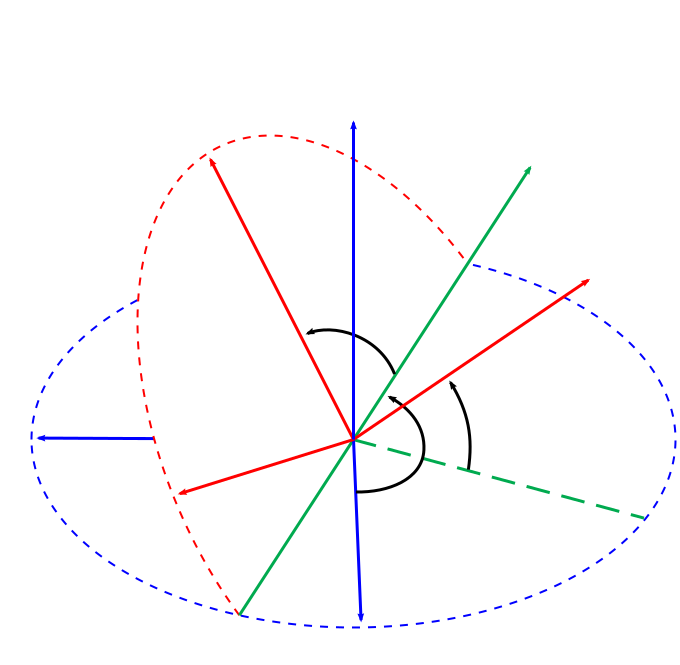
\includegraphics[width=.7\textwidth]{Images/taitbryan.pdf}};
    
\node [] at (0.5,0.2) {$\phi$};
\node [] at (0.65,-1.85) {$\psi$};
\node [] at (1.55,-0.9) {$\theta$};

\node [] at (-3.4,-1.1) {$x$};
\node [] at (0.25,-3.3) {$y$};
\node [] at (0.12,2.43) {$z$};
\node [] at (2.0,1.2) {$y^{'}$};


\node [] at (2.8,0.6) {$X$};
\node [] at (-1.5,2.05) {$Y$};
\node [] at (-2.0,-1.7) {$Z$};
\end{tikzpicture}
\caption{Representation of the body frame (red) with respect to the navigation frame (blue). The body frame was rotated, by the Euler angles $\psi, \theta, \phi$ about the axes $z, y^{'}, X$, respectively. Adapted from \cite{Wiki_taitbryan}.} \label{fig:Euler_angles}
\end{figure}

\section{Transformation Matrices}

Coordinates representing a point in one coordinate system can be transformed to another. Such a linear transformations can be expressed as multiplication of a matrix with the coordinate vector that is to be transformed. Let $\mathbf{E}$ denote the orthonormal basis $\{x, y, z\} \in \mathbb{R}^3$ and let $\mathbf{E}^{'}$ denote the orthonormal basis $\{X, Y, Z\} \in \mathbb{R}^3$. Furthermore, let $\mathbf{b}$ denote the position vector of a point in three-dimensional Euclidean space. The coordinate transformation from $\mathbf{E}$ to $\mathbf{E}^{'}$ is denoted $\bm{\Omega}_{\mathbf{E} \rightarrow \mathbf{E}^{'}}: (b_1, b_2, b3) \mapsto (b1^{'}, b2^{'}, b3^{'})$. Then, the transformation from $\mathbf{b}$ to $\mathbf{b}^{'}$ is given by

\begin{equation}\label{eq:transformation}
  \mathbf{b^{'}} = \bm{\Omega}_{\mathbf{E} \rightarrow \mathbf{E}^{'}}(\mathbf{b}) = \mathbf{T} \mathbf{b}\,,
\end{equation}

\noindent
where $\mathbf{T}$ is the transformation matrix. To transform the coordinate vector from the navigation frame to the body frame, according to the common aerospace rotation sequence mentioned above and the Nort-East-Down system (NED), the transformation matrix $C_{nb}$ is given by

\begin{equation}
\begin{split}
\mathbf{C}_{nb} & = \mathbf{T}_x(\phi) \mathbf{T}_y(\theta) \mathbf{T}_z(\psi) \\
 & = {\left[ \begin{smallmatrix}
    1 \; & 0 \; & 0 \\
    0 \; & \cos \phi \; & \sin \phi \\
    0 \; & -\sin \phi \; & \cos \phi
    \end{smallmatrix}\right]}
    {\bigg[ \begin{smallmatrix}
    \cos \theta \; & 0 \; & -\sin \theta \\
    0 \; & 1 \; & 0 \\
    \sin \theta \; & 0 \; & \cos \theta
    \end{smallmatrix} \bigg]}
    {\left[\begin{smallmatrix}
    \cos \psi \; & \sin \psi \; & 0 \\
    -\sin \psi \; & \cos \psi \; & 0 \\
    0 \; & 0 \; & 1
    \end{smallmatrix}\right]}\\
 & = {\left[\begin{smallmatrix}
   \cos \theta \cos \psi \; &
    \cos \theta \sin \psi \; &
   -\sin \theta \\
    \sin \phi \sin \theta \cos \psi - \cos \phi \sin \psi \;\; &
    \sin \phi \sin \theta \sin \psi + \cos \phi \cos \psi \;\; &
    \sin \phi \cos \theta \\
    \cos \phi \sin \theta \cos \psi + \sin \phi \sin \psi \;\; &
    \cos \phi \sin \theta \sin \psi - \sin \phi \cos \psi \;\; &
    \cos \phi \cos \theta
  \end{smallmatrix}\right]}
\end{split}
\end{equation}

\noindent
Plugged in Equation \ref{eq:transformation} ($\mathbf{T} = \mathbf{C}_{nb}$) the left multiplication of the matrices $\mathbf{T}_x(\phi), \mathbf{T}_y(\theta), \mathbf{T}_z(\psi)$ to the vector $\mathbf{b}$ represent the orthogonal projection onto the axis of the coordinate system that result from the two-dimensional rotation of $\phi, \theta, \psi$ about the axes $x, y, z$, respectively. The matrix $\mathbf{C}_{bn}$ for transforming the coordinate vector from the body frame to the navigation frame is given by

\begin{equation}
\mathbf{C}_{bn} = {\left[\begin{smallmatrix}
   \cos \theta \cos \psi \; &
    \sin \phi \sin \theta \cos \psi - \cos \phi \sin \psi \; &
    \cos \phi \sin \theta \cos \psi + \sin \phi \sin \psi \\
    \cos \theta \sin \psi \;\; &
    \sin \phi \sin \theta \sin \psi + \cos \phi \cos \psi \;\; &
    \cos \phi \sin \theta \sin \psi - \sin \phi \cos \psi \\
    -\sin \theta \;\; &
    \sin \phi \cos \theta \;\; &
    \cos \phi \cos \theta
  \end{smallmatrix}\right]}
\end{equation}

\noindent
The matrices $\mathbf{C}_{bn}$ and $\mathbf{C}_{nb}$ are known as Direct Cosine Matrices. Note that $\mathbf{C}_{bn} = \mathbf{C}^T_{nb} = \mathbf{C}^{-1}_{nb}$, so that $\mathbf{C}^{ }_{bn} \mathbf{C}_{nb} = \mathbf{I}$.  

\section{Quaternions}

\section{Projection of Gravity Vector and Earth's Magnetic Field Vector}

As described in Chapter \ref{ch:MARG}, accelerometers measure the acceleration they experience. Under static or quasi-static (steady, linear motion) conditions, or at low acceleration it can be assumed that the measured acceleration is mainly that of gravity. Be means of simple trigonometric transformations estimates for the pitch and the roll angle can be obtained. Since the gravity vector is perpendicular to the $xy$-plane and thus a rotation around the $z$-axis will not cause any variation in the sensed acceleration, the yaw angle cannot be obtained by this method. To solve this problem a three-dimensional magnetometer is used, which measures the variation of Earth's magnetic field while rotating around the $z$-axis.

\section{Integration of Angular Rate}

Another way to estimate the attitude of an object is the integration of the angular rate around the $x, y$ and $z$-axis, respectively. Although this would theoretically lead to very accurate orientation estimates, they are impaired by \gls{ARW} and dynamical bias in practice. \gls{ARW} is an effect caused by the integration of high-frequency, thermo-mechanical noise, which leads to a random additive angle in the orientation signal. An even greater impact than AWR has the gyroscopes dynamic bias, which has its origin in low-frequency flicker noise. Both effects cause a dramatical drift in the angle signal over time.

\section{Sensor Fusion}

Since the projection of the gravity vector and the Earth's magnetic field vector are only valid under static or quasi-static conditions, or at low acceleration, and the integration of the angular rate leads to non-reliable estimates due to suffering from \gls{ARW} and dynamic bias, but is not affected by the intensity of motion, a means to combine the information of both sensors is desirable. The combination of information from multiple sensors to increase the overall precision of the estimation of a certain quantity of interest is termed sensor fusion. \citeauthor{raol2009multi} \cite{raol2009multi} states the following advantages of sensor fusion:
 
\begin{itemize}
\item Robust functional and operational performance is given, in case of data loss from one sensor, due to redundancy provided by multiple sensors.
\item Enhanced confidence in the results inferred from the measurement of one sensor, if they are confirmed by the measurement of another sensor.
\item With sensor fusion an arbitrary fine time resolution of measurements is possible, whereas single sensors need a finite time to transmit measurements and so limit the frequency of measurements.
\item One sensor might be, to some extent, better in a certain state of the measured process, e.g. low or high motion intensity in attitude estimation, and thus, by fusing multiple sensor signals, a satisfactory accuracy among all states of the process could be attained.
\end{itemize}

\noindent
Sensor fusion can be realised by the use of a Kalman filter, which is described in detail in the next chapter.



	\chapter{Digital Filters}
\label{ch:digital_filters}

Conceived in general terms, a filter is a physical device for removing unwanted components of a mixture. In the technical field a filter is a system designed to extract information from noisy measurements of a process. That is, the filter delivers an estimate of the variables of principal interest, which is why it may also be called an estimator. Filter theory is applied in diverse fields of science and technology, such as communications, radar, sonar, navigation, and biomedical engineering \cite{haykin2002adaptive}.

In contrast to \emph{analogue filters} that consist of electronic circuits to attenuate unwanted frequencies in continuous-time signals and thus extract the useful signal, a \emph{digital filter} is a set of mathematical operations applied to a discrete-time signal in order to extract information about the hidden quantity of interest. A \emph{discrete-time} signal is a sequence of samples at equidistant time instants that represent the continuous-time signal with no loss, provided the sampling theorem is satisfied, according to which the sample frequency has to be greater than twice the highest frequency component of the continuous-time signal.

Digital filters can be classified as \emph{linear} and \emph{non-linear}. If the quantity at the output of the filter is a \emph{linear} function of its input, that is, the filter function satisfies the superposition principle, the filter is said to be \emph{linear}. Otherwise, the filter is \emph{non-linear}.

\section{The Filtering Problem}

Consider, as an example involving filter theory, the continuous-time dynamical system depicted in Figure \ref{fig:state_estimation}. The desired state vector of the system, $\mathbf{x}(t)$, is usually hidden and can only be observed by indirect measurements $\mathbf{y}(t)$ that are a function of $\mathbf{x}(t)$ and subject to noise. Equally, the equation describing the evolution of the state $\mathbf{x}(t)$ is usually subject to system errors. These could be caused by, for instance, effects not accounted for in the model. The dynamical system may be an aircraft in flight, in which case the elements of the state vector are constituted by its position and velocity. The measuring system may be a tracking radar producing the observation vector $\mathbf{y}(t)$ over an interval $[0, T]$. The requirement of the filter is to deliver a reliable estimate $\hat{\mathbf{x}}(t)$ of the actual state, by taking the measurement as well as prior information into account.

\tikzstyle{block} = [draw, rectangle, minimum height=3em, minimum width=6em]
\tikzstyle{output} = [coordinate]
\tikzstyle{pinstyle} = [pin edge={to-, thick, black}, align=center]

\begin{figure}
\centering
\begin{tikzpicture}[auto, thick, rounded corners=1pt, node distance=3cm,>=latex']
    \node [block, align=center, 
    	pin={[pinstyle]below:System \\ Errors}]
    	(dynamical) {Dynamical \\ system};
    \node [block, align=center, right of=dynamical, pin={[pinstyle]below:Measurement \\ errors}, node distance=4.5cm] (measuring) {Measuring \\ system};
    \node [block, align=center, right of=measuring, pin={[pinstyle]below:Prior \\ information}, node distance=4.5cm] (estimator) {Estimator};
    \node [output, right of=estimator] (output) {};
    
    \draw [->, align=center] (dynamical) -- node[name=x] {State \\ $\mathbf{x}(t)$} (measuring);
    \draw [->, align=center] (measuring) -- node[name=y] {Observation \\ $\mathbf{y}(t)$} (estimator);
    \draw [->, align=center] (estimator) -- node[name=y] {Estimate \\ of state \\ $\hat{\mathbf{x}}(t)$} (output);
\end{tikzpicture}
\caption{Block diagram depicting the components involved in state estimation, from \cite{haykin2002adaptive}.} \label{fig:state_estimation}
\end{figure}

\section{The Wiener Filter}

A statistical criterion, according to which the performance of a filter can be measured, is the mean-squared error. Consider the linear dicrete-time filter with the impulse response $w_0, w_1, w_2, \dots$ depicted in Figure \ref{fig:filtering_problem}. At some discrete time $n$ it produces an output designated by $\hat{x}(n)$, which provides an estimate of a desired response denoted by $d(n)$. According to \citeauthor{haykin2002adaptive} \cite{haykin2002adaptive} the essence of the filtering problem and the resulting requirement is summarised with the following statement:

\begin{quote}``Design a linear discrete-time filter whose output $\hat{x}(n)$ provides an estimate of the desired response $d(n)$, given a set of input samples $y(0), y(1), y(2), \dots$, such that the mean-square value of the estimation error $e(n)$, defined as the difference between the desired response $d(n)$ and the actual response $\hat{x}(n)$, is minimized.''
\end{quote}

\tikzstyle{block} = [draw, rectangle, 
    minimum height=2.6cm, minimum width=3.2cm]
\tikzstyle{sum} = [draw, circle, node distance=4cm]
\tikzstyle{input} = [coordinate]
\tikzstyle{output} = [coordinate]
\tikzstyle{error} = [coordinate]
\tikzstyle{pinstyle} = [pin edge={to-,thin,black}]

\begin{figure}
\centering
\begin{tikzpicture}[auto, thick, node distance=3cm,>=latex']
    
\node [input, name=input] {};
\node [block, rounded corners=1pt, align=left, right of=input, node distance=4.4cm] (filter) {Linear \\ discrete-time \\ filter \\ $w_0, w_1, w_2, \dots$};
\node [sum, right of=filter, node distance=4.4cm] (sum) {$\sum$};	
\node [output, right of=sum, node distance=2.8cm, name=output] {};
\node [error, below of=sum, node distance=2.8cm, name=error] {};

\draw [draw,->, align=left] (input) -- node [pos=0.29]{Input \\ $y(0), y(1), y(2), \dots$} (filter);
\draw [draw,->, align=left] (filter) -- node {Output \\ $\hat{x}(n)$} node[pos=0.9, label={below:$-$}] {} (sum);
\draw [draw,->, align=left] (output) -- node [label={above:Desired \\ response \\ $d(n)$}] {} node[pos=0.9] {$+$} (sum);
\draw [draw,->, align=left] (sum) -- node {Estimation \\ error \\ $e(n)$} (error);

\end{tikzpicture}
\caption{Block diagram representation of the statistical filtering problem, from \cite{haykin2002adaptive}.} \label{fig:filtering_problem}
\end{figure}

Assume a stationary stochastic process with known statistical parameters as the mean and correlation functions of the useful signal and the unwanted additive noise. Then, the solution to this statistical optimisation problem is commonly known as the \emph{Wiener filter}. Yet, since the Wiener filter requires a priori information about the statistics of the data to be processed, it may not be optimum for non-stationary processes. For such an environment, in which the statistics are time-varying, it needs a filter that constantly adapts its parameters to optimise its output.

\section{Adaptive Filters}

A possible approach to mitigate the limitations of the Wiener filter for non-stationary processes is the `estimate and plug' procedure. The filter `estimates' the statistical parameters of the relevant signals and `plugs' them into a \emph{non-recursive} formula for computing the filter parameters. This procedure requires excessively elaborate and costly hardware for real-time operation \cite{haykin2002adaptive}. To overcome this disadvantage one may use an \emph{adaptive filter}, which is a self-designing system that relies, in contrast, on a \emph{recursive} algorithm. This allows the filter to perform satisfactorily even if there is no complete knowledge of the relevant signal characteristics. Provided the variations in the  statistics of the input data are sufficiently slow, the algorithm can track time variations and is thus suitable for non-stationary environments. The algorithm starts from some predetermined set of initial conditions respecting the knowledge about the system. In a stationary environment it converges to the optimum Wiener solution in some statistical sense after successive iterations. The \emph{Kalman filter} is such an adaptive filter.

Due to the fact that the parameters of an adaptive filter are updated each iteration, they become data dependent. The system does not obey the principles of superposition which therefore makes the adaptive filter in reality a \emph{non-linear} system. However, an adaptive filter is commonly said to be \emph{linear} if its input-output map satisfies the superposition principle, as long as its parameters are held fixed. Otherwise it is said to be \emph{non-linear}.


\section{The Kalman Filter}

The \emph{Kalman filter} is a set of recursive mathematical equations that provides an efficient means to estimate the state of a linear dynamic system perturbed by additive white Gaussian noise, even when the precise nature of the modelled system is unknown. It incorporates knowledge of the system and measurement device dynamics, the statistical description of the system errors and measurement noise, and available information about initial conditions of the variables of interest, in order to produce an estimate of these variables, in a way that the mean of the squared error is minimised \cite{Maybeck79}. 

The filter is named after Rudolf E. Kalman who 1960 published his famous paper describing a recursive solution to the discrete-data linear filtering problem \cite{kalman_1960}. Since that time, the Kalman filter has been the subject of extensive research, due, to a large extent, to the advances in digital computing \cite{welch2014}. It finds applications in radar tracking, navigation, and orientation estimation, among others. \citeauthor{zarchan2009fundamentals} \cite{zarchan2009fundamentals} stated: ``With the possible exception of the fast Fourier transform, Kalman filtering is probably the most important algorithmic technique ever devised.''

\subsection{An Introductory Example}

The following introductory example from \citeauthor{Maybeck79} \cite{Maybeck79} is an illustrative description of the determination of a one-dimensional position to understand how the Kalman filter works. Suppose you are lost at sea during the night and take a star sighting to determine your approximate position at time $t_1$ to be $z_1$. Your location estimate is, due to inherent measurement device inaccuracies and human error, somewhat uncertain, and thus assumed to be associated with a standard deviation $\sigma_{z_1}$. The conditional probability of $x(t_1)$, your actual position at time $t_1$, conditioned on the observed value $z_1$, is depicted in Figure \ref{fig:measurement_z1}. The best estimate of your position, based on this conditional probability density, is

\begin{equation}
  \hat{x}(t_1)=z_1
\end{equation}

\noindent
and the variance of the error in the estimate is

\begin{equation}
  \sigma^2_x(t_1)=\sigma^2_{z_1}\,.
\end{equation}

\begin{figure}
\centering
\begin{tikzpicture}[pile/.style={->, >=stealth'}]

\draw[very thick] plot[samples=200, smooth, domain=-.5:8.5] (\x, {0.2+5/(1.3*sqrt(2*pi))*exp(-((\x-4)^2)/(2*1.3^2))});
  \draw[->] (-1,0) -- (9,0) node[below, pos=0.98] {$x$};
  \draw[->] (0,-0.5) -- (0,3) node[right] {$f_{x(t_1)|z(t_1)}(x|z_1)$};
  \draw[-] (4,0) -- (4,1.74) node[pos=-0.15] {$z_1$};
  \draw[pile, style={->, >=stealth', shorten <=0pt, shorten
    >=0pt}] (4,0.8) -- (2.26,0.8) node[below, pos=0.5] {$\sigma_{z_1}$};
  
\end{tikzpicture}
\caption{Conditional probability density of position based on measurement value $z_1$, from \cite{Maybeck79}.} \label{fig:measurement_z1}
\end{figure}

Right after you, say a trained navigator friend takes an independent fix at time $t_2 \cong t_1$, so that the true position has not changes at all. He obtains a measurement $z_2$ with a variance $\sigma_{z_2}$, which is somewhat smaller than yours, since he has a higher skill. Figure \ref{fig:measurement_z2} depicts the conditional density of your position at time $t_2$, based only on the measurement value $z_2$. Combining these data, your position at time $t_2 \cong t_1$, $x(t_2)$, given both $z_1$ and $z_2$, is then a Gaussian density with mean $\mu$ and variance $\sigma^2$, as indicated in Figure \ref{fig:combination}, with

\begin{figure}
\centering
\begin{tikzpicture}[pile/.style={->, >=stealth'}]

\draw[thick, dashed] plot[samples=200, smooth, domain=-.5:8.5] (\x, {0.2+5/(1.3*sqrt(2*pi))*exp(-((\x-4)^2)/(2*1.3^2))});
\draw[very thick] plot[samples=200, smooth, domain=3.9:8.1] (\x, {0.1+5/(0.6*sqrt(2*pi))*exp(-((\x-6)^2)/(2*0.6^2))});
  \draw[->] (-1,0) -- (9,0) node[below, pos=0.98] {$x$};
  \draw[->] (0,-0.5) -- (0,4) node[right] {$f_{x(t_2)|z(t_2)}(x|z_2)$};
  \draw[dashed] (4,0) -- (4,1.74) node[pos=-0.15] {$z_1$};
  \draw[pile, style={dashed, ->, >=stealth', shorten <=0pt, shorten
    >=0pt}] (4,0.8) -- (2.26,0.8) node[below, pos=0.5] {$\sigma_{z_1}$};
  \draw[-] (6,0) -- (6,3.43) node[pos=-0.08] {$z_2$};
    \draw[pile, style={->, >=stealth', shorten <=0pt, shorten
    >=0pt}] (6,2) -- (6.62,2) node[below, pos=0.5] {$\sigma_{z_2}$};
  
\end{tikzpicture}
\caption{Conditional probability density of position based on measurement value $z_2$ alone, from \cite{Maybeck79}.} \label{fig:measurement_z2}
\end{figure}

\begin{figure}
\centering
\begin{tikzpicture}[pile/.style={->, >=stealth'}]


\draw[thick, dashed] plot[samples=200, smooth, domain=-.5:8.5] (\x, {0.2+5/(1.3*sqrt(2*pi))*exp(-((\x-4)^2)/(2*1.3^2))});
\draw[thick, dashed] plot[samples=200, smooth, domain=3.9:8.1] (\x, {0.1+5/(0.6*sqrt(2*pi))*exp(-((\x-6)^2)/(2*0.6^2))});
\draw[very thick] plot[samples=200, smooth, domain=3.8:6.2] (\x, {0.05+5/(0.35*sqrt(2*pi))*exp(-((\x-5)^2)/(2*0.35^2))});
  \draw[->] (-1,0) -- (9,0) node[below, pos=0.98] {$x$};
  \draw[->] (0,-0.5) -- (0,6) node[right] {$f_{x(t_2)|z(t_2)}(x|z_2)$};
  \draw[dashed] (4,0) -- (4,1.74) node[pos=-0.15] {$z_1$};
  \draw[pile, style={dashed, ->, >=stealth', shorten <=0pt, shorten
    >=0pt}] (4,0.8) -- (2.26,0.8) node[below, pos=0.5] {$\sigma_{z_1}$};
  \draw[dashed] (6,0) -- (6,3.43) node[pos=-0.08] {$z_2$};
    \draw[pile, style={dashed, ->, >=stealth', shorten <=0pt, shorten
    >=0pt}] (6,2) -- (6.61,2) node[below, pos=0.5] {$\sigma_{z_2}$};
  \draw[-] (5,0) -- (5,5.75) node[pos=-0.05] {$\mu$};
    \draw[pile, style={->, >=stealth', shorten <=0pt, shorten
    >=0pt}] (5,3.5) -- (4.67,3.5) node[below, pos=0.5] {$\sigma$};
  
\end{tikzpicture}
\caption{Conditional probability density of position based on data $z_1$ and $z_2$, from \cite{Maybeck79}.} \label{fig:combination}
\end{figure}


\begin{equation}\label{eq:mu}
  \mu=z_1\frac{\sigma^2_{z_2}}{\sigma^2_{z_1}+\sigma^2_{z_2}}+z_2\frac{\sigma^2_{z_1}}{\sigma^2_{z_1}+\sigma^2_{z_2}}
\end{equation}

\noindent
and

\begin{equation}
  \frac{1}{\sigma^2}=\frac{1}{\sigma^2_{z_1}}+\frac{1}{\sigma^2_{z_2}}\,.
\end{equation}

\noindent
The uncertainty in your estimate of position has been decreased because $\sigma$ is less than either $\sigma^2_{z_1}$ or $\sigma^2_{z_2}$. Even if $\sigma_{z_1}$ was very large, the variance of the estimate is less than $\sigma_{z_2}$, which means that even poor quality data increases the precision of the filter output. The best estimate, given this density, is

\begin{equation}\label{eq:filter_output}
  \hat{x}(t_2)=\mu\,,
\end{equation}

\noindent
with an associated error variance $\sigma^2$.

Having a closer look at the form of $\mu$ in Equation \ref{eq:mu}, one notices that it makes good sense. If the measurements were of equal precision, meaning $\sigma_{z_1}=\sigma_{z_2}$, the optimal estimate is simply the average of both measurements, as would be expected. If $\sigma_{z_1}$ is larger than $\sigma_{z_2}$, the equation weights $z_2$ more heavily than $z_1$.

Equation \ref{eq:filter_output} for the filter output can be written as

\begin{equation}\label{eq:x2_hat}
\begin{split}
  \hat{x}(t_2) & =z_1\frac{\sigma^2_{z_2}}{\sigma^2_{z_1}+\sigma^2_{z_2}}+z_2\frac{\sigma^2_{z_1}}{\sigma^2_{z_1}+\sigma^2_{z_2}} \\
  & =z_1+\frac{\sigma^2_{z_1}}{\sigma^2_{z_1}+\sigma^2_{z_2}}[z_2-z_1]
\end{split}
\end{equation}

\noindent
or in a form that is used in Kalman filter implementations, with $\hat{x}(t_1)=z_1$, as

\begin{equation}\label{eq:x2_hat_kalman}
  \hat{x}(t_2) = \hat{x}(t_1) + K(t_2)[z_2-\hat{x}(t_1)]\,,
\end{equation}

\noindent
where

\begin{equation}\label{}
  K(t_2) = \frac{\sigma^2_{z_1}}{\sigma^2_{z_1}+\sigma^2_{z_2}}\,.
\end{equation}

\noindent
These equation represent the `predictor-corrector' structure of the Kalman filter. A prediction of the value that the desired variables and the measurements will have at the next measurement time is made, based on all previous information. Then the difference between the measurement and its predicted value is used to correct the prediction of the desired variables. According to Equation \ref{eq:x2_hat_kalman} the optimal estimate at time $t_2$, $\hat{x}(t_2)$, is equal to $\hat{x}(t_1)$, the best prediction of its value before $z_2$ is taken, plus a correction term of an optimal weighting value times the difference between $z_2$ and the best prediction of it before the measurement is actually taken.

To incorporate dynamics into the model, suppose you travel for some time before taking another measurement. The best model you have for your motion may be of the form

\begin{equation}\label{}
  \frac{dx}{dt} = u + w\,,
\end{equation}

\noindent
where $u$ is a nominal velocity and $w$ is a noise term, representing the uncertainty in your knowledge of the actual velocity due to disturbances and effects not accounted for in the simple first order equation. It will be modelled as white Gaussian noise with a mean of zero and variance of $\sigma^2_w$.

\begin{figure}
\centering
\begin{tikzpicture}[pile/.style={->, >=stealth'}]

  \draw[very thick] plot[samples=200, smooth, domain=0.8:3.2] (\x, {0.05+5/(0.35*sqrt(2*pi))*exp(-((\x-2)^2)/(2*0.35^2))});
  \draw[very thick] plot[samples=200, smooth, domain=2.2:7.8] (\x, {0.2+5/(0.7*sqrt(2*pi))*exp(-((\x-5)^2)/(2*0.7^2))});
  \draw[very thick] plot[samples=200, smooth, domain=4.5:11.5] (\x, {0.4+5/(1.3*sqrt(2*pi))*exp(-((\x-8)^2)/(2*1.3^2))});

  \draw[->] (-0.5,0) -- (12,0) node[below, pos=0.98] {$x$};
  \draw[->] (0,-0.5) -- (0,6.5) node[right] {$f_{x(t)|z(t_1), z(t_2)}(x|z_1, z_2)$};
  \draw[-] (8,0) -- (8,1.94) node[pos=-0.15] {$\hat{x}(t^-_3)$};
  \draw[pile, style={->, >=stealth', shorten <=0pt, shorten
    >=0pt}] (8,0.8) -- (10.07,0.8) node[below, pos=0.5] {$\sigma_x(t^-_3)$};
  \draw[-] (5,0) -- (5,3.07) node[pos=-0.09] {$\hat{x}(t)$};
  \draw[pile, style={->, >=stealth', shorten <=0pt, shorten
    >=0pt}] (5,2) -- (5.65,2) node[right, pos=0.98] {$\sigma_x(t)$};
  \draw[-] (2,0) -- (2,5.75) node[pos=-0.05] {$\hat{x}(t_2)$};
  \draw[pile, style={->, >=stealth', shorten <=0pt, shorten
    >=0pt}] (2,3.5) -- (2.33,3.5) node[right, pos=0.95] {$\sigma_x(t_2)$};
 
  \draw[pile, style={dashed, ->, >=stealth', shorten <=0pt, shorten
    >=0pt}] (2,4) -- (8,4) node[above, pos=0.75] {$u[t_3-t_2]$};
  
\end{tikzpicture}
\caption{Propagation of conditional probability density, from \cite{Maybeck79}.} \label{fig:propagation}
\end{figure}

The conditional density of the position at time $t_2$, given $z_1$ and $z_2$, was previously derived. Figure \ref{fig:propagation} shows graphically how the density travels along the x-axis as time progresses. It start at the best estimate and moves according to the above mentioned model of dynamics. Due to the constant addition of uncertainty over time it spreads out. As the variance becomes greater you become less sure of your position. The Gaussian density $f_{x(t_3)|z(t_1), z(t_2)}(x|z_1, z_2)$ can be expressed mathematically by its mean and variance given by

\begin{equation}\label{eq:system_model}
  \hat{x}(t^-_3)=\hat{x}(t_2)+u[t_3-t_2]\,,
\end{equation}

\begin{equation}\label{eq:variance_predicted}
  \sigma^2_x(t^-_3)=\sigma^2_x(t_2)+\sigma^2_w[t_3-t_2]\,.
\end{equation}

\noindent
Before the measurement is taken at $t_3$, $\hat{x}(t^-_3)$ is the optimal prediction of the location at $t^-_3$, associated with the variance $\sigma^2_x(t^-_3)$ in this prediction.

Now a measurement $z_3$ with an assumed variance $\sigma^2_{z_3}$ is taken. As before, its conditional probability density is combined with the density with mean $\hat{x}(t^-_3)$ and variance $\sigma^2_x(t^-_3)$, to yield a Gaussian density with mean

\begin{equation}\label{eq:estimation_kalman}
  \hat{x}(t_3) = \hat{x}(t^-_3) + K(t_3)[z_3-\hat{x}(t^-_3)]
\end{equation}

\noindent
and variance

\begin{equation}\label{eq:variance_kalman}
  \sigma^2_x(t_3) = \sigma^2_x(t^-_3)-K(t_3)\sigma^2_x(t^-_3)\,,
\end{equation}

\noindent
where the gain $K(t_3)$ is given by

\begin{equation}\label{eq:gain_kalman}
  K(t_3) = \frac{\sigma^2_x(t^-_3)}{\sigma^2_x(t^-_3)+\sigma^2_{z_3}}\,.
\end{equation}

Observing the form of Equation \ref{eq:gain_kalman} the reasonableness of the filter structure becomes obvious. If the variance of the measurement noise $\sigma^2_{z_3}$ is large, then $K(t_3)$ is small, meaning that little confidence is put in a very noisy measurement and that it is weighted lightly. For $\sigma^2_{z_3}\rightarrow\infty$, $K(t_3)$ becomes zero, and $\hat{x}(t_3)$ equals $\hat{x}(t^-_3)$. Thus, an infinitely noisy measurement is totally ignored. Likewise, if the dynamical system noise variance $\sigma^2_w$ is large, then according to Equation \ref{eq:variance_predicted}, $\sigma^2_x(t^-_3)$ will be large, and so will be $K(t_3)$. Therefore, the measurement is weighted heavily, in case you are not very certain about the output of the system model within the filter structure. In the limit as $\sigma^2_w \rightarrow\infty$, $\sigma^2_x(t^-_3) \rightarrow\infty$, and $K(t_3) \rightarrow1$, so Equation \ref{eq:filter_output} yields

\begin{equation}\label{eq:prediction_kalman}
  \hat{x}(t_3) = \hat{x}(t^-_3) + 1 \cdot [z_3-\hat{x}(t^-_3)] = z_3\,.
\end{equation}

\noindent
That means that in the limit of absolutely no confidence in the system model output, solely the new measurement is taken as the optimal estimate. Finally, if you are absolutely sure of your estimate before $z_3$ comes available, $\sigma^2_x(t^-_3)$ would become zero, and so would $K(t_3)$, which means that the measurements would be left disregarded. 

Extending Equations \ref{eq:system_model}, \ref{eq:variance_predicted}, \ref{eq:estimation_kalman}, \ref{eq:variance_kalman}, and \ref{eq:gain_kalman} to the vector case, and allowing time varying parameters in the system and noise description leads to the general Kalman filter equations. A complete mathematical derivation is found in \citeauthor{haykin2002adaptive} \cite{haykin2002adaptive}.

\subsection{Formulation of the Kalman Filter Equations} \label{sec:Kalman_equations}

Let $\mathbf{x}_k \in \mathbb{R}^n$ be the state vector of a discrete-time controlled process governed by the linear stochastic difference equation 

\begin{equation}\label{eq:time_dynamical_system_plant}
  \mathbf{x}_k = \bm{\Phi}_{k-1}\mathbf{x}_{k-1}+\mathbf{B}_{k-1}\mathbf{u}_{k-1}+\mathbf{w}_{k-1}
\end{equation}

\noindent
and $\mathbf{z}_k \in \mathbb{R}^m$ the observation or measurement vector of this process, given by

\begin{equation}\label{eq:time_dynamical_system_measurement}
  \mathbf{z}_k = \mathbf{H}_{k}\mathbf{x}_{k}+\mathbf{v}_{k}\,,
\end{equation}

\noindent
where the index $k \in \mathbb{N}^0$ denotes discrete time normalised to the sampling interval. The $n\times1$ vector $w_k$ and the $m\times1$ vector $v_k$ represent the process noise and the measurement noise, respectively, modelled as zero-mean, Gaussian white noise

\begin{equation}\label{eq:process_noise}
  \mathbf{w}_{k} \sim \mathcal{N}(0,\mathbf{Q}_k)\,,
\end{equation}

\begin{equation}\label{eq:measurement_noise}
  \mathbf{v}_{k} \sim \mathcal{N}(0,\mathbf{R}_k)\,,
\end{equation}
 
\noindent
with the process noise covariance matrix $\mathbf{Q}_k$ and the measurement noise covariance matrix $\mathbf{R}_k$. The $n\times n$ transition matrix $\bm{\Phi}_{k-1}$ in \ref{eq:time_dynamical_system_plant} relates the state at the previous time step $k-1$ to the state at the current step $k$. The $n\times l$ matrix $\mathbf{B}_{k-1}$ relates the known, optional control input $\mathbf{u}_{k-1} \in \mathbb{R}^l$ to the state $\mathbf{x}_k$. Finally, the $m\times n$ measurement matrix $\mathbf{H}_{k}$ in \ref{eq:time_dynamical_system_measurement} relates the state $\mathbf{x}_k$ to the measurement $\mathbf{z}_k$. Both noise processes are assumed to be uncorrelated. The process noise might not always have a physical meaning. However, it represents the fact that the model of the real world is not precise. The process and measurement noise covariance matrices are related to the respective noise vectors according to

\begin{equation}
  \mathbf{Q}_k = \mbox{E}[\mathbf{w}_{k},\mathbf{w}^T_{k}]\,,
\end{equation}

\begin{equation}
  \mathbf{R}_k = \mbox{E}[\mathbf{v}_{k},\mathbf{v}^T_{k}]\,,
\end{equation}

\noindent
where E denotes the expected value.

The Kalman filter solves the problem of estimating the state $\mathbf{x}_k$ of the given linear stochastic system, minimising the weighted mean-squarred error. The state estimate is denoted with $\hat{\mathbf{x}}_k$, which is also a linear function of the measurement $\mathbf{z}_k$. This problem is called the \emph{linear quadratic Gaussian} estimation problem; the dynamic system is linear, the performance cost function is quadratic, and the random process is Gaussian.

We define the vector $\hat{\mathbf{x}}^-_k \in \mathbb{R}^n$ as the \emph{a priori} state estimate representing knowledge of the process prior to step $k$ and $\hat{\mathbf{x}}_k \in \mathbb{R}^n$ as the \emph{a posteriori} state estimate at step $k$ given the measurement $\mathbf{z}_k$:

\begin{equation}\label{eq:apriori_estimate}
  \hat{\mathbf{x}}^-_k = \bm{\Phi}_{k-1}\hat{\mathbf{x}}_{k-1}+\mathbf{B}_{k-1}\mathbf{u}_{k-1}\,,
\end{equation}

\begin{equation}\label{eq:aposteriori_estimate}
  \hat{\mathbf{x}}_k = \hat{\mathbf{x}}^-_k + \mathbf{K}_{k}[\mathbf{z}_k-\mathbf{H}_{k}\hat{\mathbf{x}}^-_k]\,.
\end{equation}

\noindent
The term $[\mathbf{z}_k-\mathbf{H}_{k}\hat{\mathbf{x}}^-_k]$ is called the measurement \emph{innovation} or \emph{residual}. It reflects the discordance between the predicted measurement $\mathbf{H}_{k}\hat{\mathbf{x}}^-_k$ and the actual measurement $\mathbf{z}_k$. The $n\times m$ matrix $\mathbf{K}_{k}$ is termed the Kalman gain and is given by

\begin{equation}\label{eq:Kalman_gain}
  \mathbf{K}_{k} = \mathbf{P}^-_k \mathbf{H}^T_k[\mathbf{H}_k \mathbf{P}^-_k \mathbf{H}^T_k + \mathbf{R}_k]^{-1}\,,
\end{equation}

\noindent
with

\begin{equation}\label{eq:apriori_error_cov}
  \mathbf{P}^-_{k} = \bm{\Phi}_{k-1} \mathbf{P}_{k-1} \bm{\Phi}^T_{k-1} + \mathbf{Q}_{k-1}
\end{equation}

\noindent
and

\begin{equation}\label{eq:aposteriori_error_cov}
  \mathbf{P}_{k} = [\mathbf{I} - \mathbf{K}_{k}\mathbf{H}_{k}]\mathbf{P}^-_{k}\,.
\end{equation}

\noindent
Figure \ref{fig:kalman_filter_model} illustrates the relation of the Kalman filter to the discrete-time dynamical system, where $z^{-1}$ denotes the unit-delay and $\mathbf{I}$ the $n\times n$ identity matrix. For the sake of simplicity the control input is not depicted.

\tikzstyle{block} = [draw, rectangle, minimum height=0.8cm, minimum width=0.8cm]
\tikzstyle{sum} = [draw, circle]
\tikzstyle{output} = [coordinate]
\tikzstyle{input} = [coordinate]

\begin{figure}
\centering
\resizebox{13.5cm}{!}{
\begin{tikzpicture}[auto, thick, node distance=1.5cm,>=latex']
	
	\node [sum] (sum1) {$\sum$};
	\node [input, above of=sum1] (w) {};
    \node [block, align=center, 
    	right of=sum1, node distance=3cm] (H) {$\mathbf{H}_k$};
    \node [block, align=center, below of=sum1, node distance=1.8cm] (phi) {$\bm{\Phi}_{k-1}$};
    \node [sum, right of=H, node distance=1.5cm] (sum2) {$\sum$};
    \node [sum, right of=sum2, node distance=1.8cm] (sum3) {$\sum$};
    \node [input, above of=sum2] (v) {};
    \node [block, align=center, 
    	right of=sum3, node distance=1.5cm] (K) {$\mathbf{K}_k$};
    \node [block, align=center, below of=K, node distance=1.8cm] (H1) {$\mathbf{H}_k$};
    \node [block, align=center, right of=H1, node distance=2.5cm] (phi1) {$\bm{\Phi}_{k-1}$};
    \node [block, align=center, right of=phi1, node distance=2.2cm] (delay1) {$z^{-1_{ }}\mathbf{I}$};
    \node [sum, right of=K, node distance=1.5cm] (sum4) {$\sum$};
    \node [output, right of=sum4, node distance=4.0cm] (out) {};
    
    
    \draw [->] (sum1) -- node[] {$\mathbf{x}_k$} node[name=x_k, pos=0.8] {} (H);
    \node [block, below of=x_k, node distance=1.93cm] (delay) {$z^{-1_{ }}\mathbf{I}$};
    \draw [->, align=center] (delay) -- node [label={below:$\mathbf{x}_{k-1}$}, pos=0.4] {} (phi);
    \draw [->] (phi) -- node[pos=0.87] {$+$} (sum1);
    \draw [->] (H) -- node[label={below:$+$}, pos=0.77] {} (sum2);
    \draw [->] (sum2) -- node[] {$\mathbf{z}_k$} node[label={below:$+$}, pos=0.79] {} (sum3);
    \draw [->] (sum3) -- node[label={below:$+$}, pos=0.65] {} (K);
    \draw [->] (w) -- node [label={left:$\mathbf{w}_{k-1}$}, pos=0.29]{} node[label={left:$+$}, pos=0.88] {} (sum1);
    \draw [->] (v) -- node [label={left:$\mathbf{v}_{k}$}, pos=0.29]{} node[label={left:$+$}, pos=0.88] {} (sum2);
    \draw [->] (x_k) -- (delay);
    \draw [->] (H1) -| node[pos=0.89] {$-$} (sum3);
    \draw [->] (K) -- node[label={below:$+$}, pos=0.77] {} (sum4);
    \draw [->] (phi1) -- node[pos=0.27, name=h-phi] {} node[] {$\hat{\mathbf{x}}^-_k$} (H1);
    \draw [->] (delay1) -- node[] {$\hat{\mathbf{x}}_{k-1}$} node[] {} (phi1);
     \draw [->] (h-phi) -- node[pos=0.90] {$+$} (sum4);
     \draw [->] (sum4) -- node[pos=0.77, name=xk_hat] {$\hat{\mathbf{x}}_k$} (out);
     \draw [->] (xk_hat) -- (delay1);
     
\end{tikzpicture}
}

\caption{Block diagram depicting the relation between a discrete-time dynamical system, its observation, and the Kalman filter.} \label{fig:kalman_filter_model}
\end{figure}

The Kalman filter equations can be divided into two groups: \emph{time update} Equations \ref{eq:apriori_estimate}, \ref{eq:apriori_error_cov} and \emph{measurement update} Equations \ref{eq:aposteriori_estimate} , \ref{eq:Kalman_gain}, and \ref{eq:aposteriori_error_cov}, as seen in Figure \ref{fig:kalman_filter_cycle}, which shows the `predict and correct' behaviour of the filter algorithm. After an initialisation of the parameters, the \emph{time update} and \emph{measurement update} steps are repeated recursively every time step.


\tikzstyle{block} = [draw, rectangle, thick, 
    minimum height=1.5cm, minimum width=8cm]
\tikzstyle{output} = [coordinate]

\begin{figure}[t]
\centering
\begin{tikzpicture}[auto, rounded corners=1pt, node distance=4cm,>=latex']
    
\node [block, align=center] (init) {Initialisation of parameters \\[3mm] $\mathbf{P}_{0}, \mathbf{x}_{0}, \mathbf{H}_{0}, \bm{\Phi}_{0}, \mathbf{Q}_{0}, \mathbf{R}_{0},$};
\node [block, align=center, below of=init, node distance=3.2cm] (predict) {\emph{Time update} \\[3mm] Compute \emph{a priori} estimate: \\ $\hat{\mathbf{x}}^-_k = \bm{\Phi}_{k-1}\hat{\mathbf{x}}_{k-1}+\mathbf{B}_{k-1}\mathbf{u}_{k-1}$ \\ Compute \emph{a priori} error covariance: \\ $\mathbf{P}^-_{k} = \bm{\Phi}_{k-1} \mathbf{P}_{k-1} \bm{\Phi}^T_{k-1} + \mathbf{Q}_{k-1}$};
\node [block, align=center, below of=predict, node distance=4.3cm] (update) {\emph{Measurement update} \\[3mm] Compute Kalman gain: \\ $\mathbf{K}_{k} = \mathbf{P}^-_k \mathbf{H}^T_k[\mathbf{H}_k \mathbf{P}^-_k \mathbf{H}^T_k + \mathbf{R}_k]^{-1}$ \\ Compute \emph{a posteriori} estimate: \\ $\hat{\mathbf{x}}_k = \hat{\mathbf{x}}^-_k + \mathbf{K}_{k}[\mathbf{z}_k-\mathbf{H}_{k}\hat{\mathbf{x}}^-_k]$ \\ Update error covariance: \\ $\mathbf{P}_{k} = [\mathbf{I} - \mathbf{K}_{k}\mathbf{H}_{k}]\mathbf{P}^-_{k}$};
\node [output, below of=update, node distance=3cm, name=output] {Output};
\node [output, below of=update, node distance=2.5cm, name=help1] {};
\node [output, right of=help1, node distance=4.7cm, name=help2] {};
\node [output, below of=init, node distance=1.16cm, name=help4] {};
\node [output, right of=help4, node distance=4.7cm, name=help3] {};

\draw [draw,-stealth, thick, align=left] (init) -- (predict);
\draw [draw,-stealth, thick, align=left] (predict) -- (update);
\draw [draw,-stealth, thick, align=left] (update) -- node [label={left:Output}]{} (output);
\draw [draw,-stealth, thick] (help1) -- (help2) -- (help3) -- (help4);
\end{tikzpicture}
\caption{Operation cycle of the Kalman filter algorithm illustrating `predict and correct' behaviour.} \label{fig:kalman_filter_cycle}
\end{figure}


\subsection{The Extended Kalman Filter}

Up to this point the Kalman filter has solved the filtering problem for \emph{linear} time-dynamical systems. One may extend the Kalman filter to systems with state dynamics governed by \emph{non-linear} state transformations

\begin{equation}\label{eq:time_dynamical_system_plant_extended}
  \mathbf{x}_k = \bm{\phi}_{k-1}(\mathbf{x}_{k-1}, \mathbf{u}_{k-1})+\mathbf{w}_{k-1}, \quad \mathbf{w}_{k} \sim \mathcal{N}(0,\mathbf{Q}_k)\,,
\end{equation}

\noindent
and/or a \emph{non-linear} transformation from state variables to measurement variables

\begin{equation}\label{eq:time_dynamical_system_measurement_extended}
  \mathbf{z}_k = \mathbf{h}_{k}(\mathbf{x}_{k})+\mathbf{v}_{k}, \quad \mathbf{v}_{k} \sim \mathcal{N}(0,\mathbf{R}_k)\,.
\end{equation}

\noindent
The \emph{functional} $\bm{\phi}_{k-1}$ denotes the \emph{non-linear} transition matrix function that may be time varying. It relates the state at the previous time step $k-1$ to the current time step $k$. The vector $\mathbf{u}_{k-1}$ is again the exogenous control input. The functional $\mathbf{h}_{k}$ denotes a \emph{non-linear} measurement matrix function that relates the state $\mathbf{x}_{k}$ to the measurement $\mathbf{z}_k$ and is possibly time varying, too.

Some non-linear problems can be deemed \emph{quasilinear}, which means that the variation of the non-linear functionals $\bm{\phi}$ and $\mathbf{h}$ are predominantly linear about the value $\mathbf{x}_0$. That is,

\begin{equation}\label{eq:linear_phi}
  \bm{\phi}_{k}(\mathbf{x}_0 + d \mathbf{x}, \mathbf{u}) \approx \bm{\phi}_{k}(\mathbf{x}_0, \mathbf{u}) + d \mathbf{x} \left. \frac{\partial \bm{\phi}_{k}(\mathbf{x}, \mathbf{u})}{\partial \mathbf{x}} \right|_{\mathbf{x}_0, \mathbf{u}}\,,
\end{equation}

\begin{equation}\label{eq:linear_h}
  \mathbf{h}_{k}(\mathbf{x}_0 + d \mathbf{x}) \approx \mathbf{h}_{k}(\mathbf{x}_0) + d \mathbf{x} \left. \frac{\partial \mathbf{h}_{k}(\mathbf{x})}{\partial \mathbf{x}} \right|_{\mathbf{x}_0}\,,
\end{equation}

\noindent
which requires that $\bm{\phi}$ and $\mathbf{h}$ are differentiable at $\mathbf{x}$.

Through a \emph{linearisation} of the state-space model of Equations \ref{eq:time_dynamical_system_plant_extended} and \ref{eq:time_dynamical_system_measurement_extended} at each time instant around the most recent state estimate, the standard Kalman filter equation from Section \ref{sec:Kalman_equations} can be applied. The filter resulting from a \emph{linear approximation} of the state transitions and the relation of the measurement to the respective state is referred to as the \emph{extended Kalman filter} (EKF).

Similar to Equation \ref{eq:apriori_estimate}, the predicted state estimate is given by

\begin{equation}\label{eq:apriori_estimate_extended}
  \hat{\mathbf{x}}^{-}_k = \bm{\phi}_{k-1}(\mathbf{x}_{k-1}, \mathbf{u}_{k-1})\,,
\end{equation}

\noindent
and the predicted measurement by

\begin{equation}\label{eq:predicted_measurement_extended}
  \hat{\mathbf{z}}_k = \mathbf{h}_{k}(\hat{\mathbf{x}}^{-}_{k})\,.
\end{equation}

\noindent
The \emph{a posteriori} estimate is then, conditioned on the actual measurement, 

\begin{equation}\label{eq:aposteriori_estimate_extended}
  \hat{\mathbf{x}}_k = \hat{\mathbf{x}}^-_k + \mathbf{K}_{k}[\mathbf{z}_k-\hat{\mathbf{z}}_k]\,.
\end{equation}

\noindent
The corresponding \emph{a priori} covariance matrix $\mathbf{P}^-_{k}$, the Kalman gain $\mathbf{K}_{k}$, and the \emph{a posteriori} covariance matrix $\mathbf{P}_{k}$ are equal to Equations \ref{eq:Kalman_gain}, \ref{eq:apriori_error_cov}, and \ref{eq:aposteriori_error_cov} in Section \ref{sec:Kalman_equations}. They are reproduced here with the linearised state transition and measurement matrices for convenience of presentation:

\begin{equation}\label{eq:apriori_error_cov_extended}
  \mathbf{P}^-_{k} = \bm{\Phi}^{[1]}_{k-1} \mathbf{P}_{k-1} \bm{\Phi}^{[1]T}_{k-1} + \mathbf{Q}_{k-1}\,,
\end{equation}

\begin{equation}\label{eq:Kalman_gain_extended}
  \mathbf{K}_{k} = \mathbf{P}^-_k \mathbf{H}^{[1]T}_k[\mathbf{H}^{[1]}_k \mathbf{P}^-_k \mathbf{H}^{[1]T}_k + \mathbf{R}_k]^{-1}\,,
\end{equation}

\begin{equation}\label{eq:aposteriori_error_cov_extended}
  \mathbf{P}_{k} = [\mathbf{I} - \mathbf{K}_{k}\mathbf{H}^{[1]}_{k}]\mathbf{P}^-_{k}\,.
\end{equation}

\noindent
The Jacobian matrices of the functionals $\bm{\phi}$ and $\mathbf{h}$ are given by  

\begin{equation}\label{eq:Phi_first_order}
  \bm{\Phi}^{[1]}_{k-1} =  \left. \frac{\partial \bm{\phi}_{k-1}(\mathbf{x}, \mathbf{u})}{\partial \mathbf{x}} \right|_{\mathbf{x}=\hat{\mathbf{x}}^-_{k-1}, \mathbf{u}_{k-1}} \,,
\end{equation}
and
\begin{equation}\label{eq:Phi_first_order}
  \mathbf{H}^{[1]}_{k} = \left. \frac{\partial \mathbf{h}_{k}(\mathbf{x})}{\partial \mathbf{x}} \right|_{\mathbf{x}=\hat{\mathbf{x}}^-_{k}} \,.
\end{equation}

\noindent
The $ij$\textsuperscript{th} entry of $\bm{\Phi}^{[1]}_{k-1}$ is equal to the partial derivative of the $i$\textsuperscript{th} component of $\bm{\phi}_{k-1}(\mathbf{x})$ with respect to the $j$\textsuperscript{th} component of $\mathbf{x}$. The derivatives are evaluated at $\mathbf{x}=\hat{\mathbf{x}}^-_{k-1}$. Likewise, the $ij$\textsuperscript{th} entry of $\mathbf{H}^{[1]}_{k-1}$ is equal to the partial derivative of the $i$\textsuperscript{th} component of $\mathbf{h}_{k}(\mathbf{x})$ with respect to the $j$\textsuperscript{th} component of $\mathbf{x}$. The derivatives are evaluated at $\mathbf{x}=\hat{\mathbf{x}}^-_{k}$. The superscript $^{[1]}$ denotes the \emph{first-order} approximation.

Figure \ref{fig:extended_kalman_filter_cycle} illustrates the `predict and correct' behaviour of the extended Kalman filter algorithm. Likewise, after an initialisation of the parameters, the \emph{time update} and \emph{measurement update} steps are repeated recursively every time step. In addition to the standard Kalman filter equations, the Jacobian matrices have to be computed, in order to linearise the state-space model at each time instant around the most recent state estimate.

\tikzstyle{block} = [draw, rectangle, thick, 
    minimum height=1.5cm, minimum width=8cm]
\tikzstyle{output} = [coordinate]

\begin{figure}[t]
\centering
\begin{tikzpicture}[auto, rounded corners=1pt, node distance=5cm,>=latex']
    
\node [block, align=center] (init) {Initialisation of parameters \\[3mm] $\mathbf{P}_{0}, \mathbf{x}_{0}, \mathbf{H}^{[1]}_{0}, \bm{\Phi}^{[1]}_{0}, \mathbf{Q}_{0}, \mathbf{R}_{0},$};
\node [block, align=center, below of=init, node distance=4cm] (predict) {\emph{Time update} \\[3mm] Compute \emph{a priori} estimate: \\ $\hat{\mathbf{x}}^{-}_k = \bm{\phi}_{k-1}(\mathbf{x}_{k-1}, \mathbf{u}_{k-1})$ \\ Compute Jacobian matrix: \\ $\bm{\Phi}^{[1]}_{k-1} =  \left. \frac{\partial \bm{\phi}_{k-1}(\mathbf{x}, \mathbf{u})}{\partial \mathbf{x}} \right|_{\mathbf{x}=\hat{\mathbf{x}}^-_{k-1}, \mathbf{u}_{k-1}}$ \\ Compute \emph{a priori} error covariance: \\ $\mathbf{P}^-_{k} = \bm{\Phi}^{[1]}_{k-1} \mathbf{P}_{k-1} \bm{\Phi}^{[1]T}_{k-1} + \mathbf{Q}_{k-1}$};
\node [block, align=center, below of=predict, node distance=5.8cm] (update) {\emph{Measurement update} \\[3mm] Compute Jacobian matrix: \\ $\mathbf{H}^{[1]}_{k} = \left. \frac{\partial \mathbf{h}_{k}(\mathbf{x})}{\partial \mathbf{x}} \right|_{\mathbf{x}=\hat{\mathbf{x}}^-_{k}}$ \\ Compute Kalman gain: \\ $\mathbf{K}_{k} = \mathbf{P}^-_k \mathbf{H}^{[1]T}_k[\mathbf{H}^{[1]}_k \mathbf{P}^-_k \mathbf{H}^{[1]T}_k + \mathbf{R}_k]^{-1}$ \\ Compute \emph{a posteriori} estimate: \\ $\hat{\mathbf{x}}_k = \hat{\mathbf{x}}^-_k + \mathbf{K}_{k}[\mathbf{z}_k-\mathbf{h}_{k}(\hat{\mathbf{x}}^-_k)]$ \\ Update error covariance: \\ $\mathbf{P}_{k} = [\mathbf{I} - \mathbf{K}_{k}\mathbf{H}^{[1]}_{k}]\mathbf{P}^-_{k}$};
\node [output, below of=update, node distance=3.8cm, name=output] {Output};
\node [output, below of=update, node distance=3.35cm, name=help1] {};
\node [output, right of=help1, node distance=4.7cm, name=help2] {};
\node [output, below of=init, node distance=1.23cm, name=help4] {};
\node [output, right of=help4, node distance=4.7cm, name=help3] {};

\draw [draw,-stealth, thick, align=left] (init) -- (predict);
\draw [draw,-stealth, thick, align=left] (predict) -- (update);
\draw [draw,-stealth, thick, align=left] (update) -- node [label={left:Output}]{} (output);
\draw [draw,-stealth, thick] (help1) -- (help2) -- (help3) -- (help4);
\end{tikzpicture}
\caption{Operation cycle of the extended Kalman filter algorithm illustrating `predict and correct' behaviour.} \label{fig:extended_kalman_filter_cycle}
\end{figure}

Extended Kalman filtering is commonly used. In fact, it was the first successful application of the Kalman filter \cite{grewal2008kalman}. Unlike its linear counterpart, the extended Kalman filter may not necessarily be an optimal estimator. Owing to its linearisation the EKF may quickly diverge, if the process is modelled incorrectly or the initial state estimate is wrong.



	\chapter{Implementation}
\label{ch:Implementation}

This chapter describes the implementation and applies the fundamentals acquired in the previous the chapters.

\section{Initial Situation}

\section{Theoretical Design}

\section{Implementation}

\section{Experiments}

\section{Results}

\section{Discussion}


	\chapter{Conclusion and Future Work}
\label{ch:Conclusion and Future Work}

\section{Conclusions}

Gait analysis is a useful tool both in clinical practice and biomechanical research. In this work I implemented an extended Kalman filter along with some auxiliary routines that . and showed that motion-based acceleration correction can improve the angle estimates during faster motion. In order to replace a camera-based motion capture system with low cost wearable MARG sensors, some technical deails need to be improved. One could use a more complex mathematical model of the leg that takes motions outside 

Summarising the above, I can say that I have learned a lot in the four month that I spent in Granada. Amongst others I have come to know many new work methods, not only due to being exposed to people from a different culture, but also due to the fact that scientific research differs strongly from the work as a student at university. I gained a deeper understanding of orientation estimation and how Kalman filtering  benefits the accuracy. I improved my MATLAB$\textsuperscript{\textregistered}$ skills and I am now familiar with tools such as GitHub and Pivotal Tracker which make working in a team much easier and significantly more efficient.  While working at the research centre, I obtained a valuable insight into scientific research and could improve my oral and written English skills. Furthermore I now know the fundamentals of \LaTeX{}.

All in all it was a great experience, professionally as well as personally. I truly and unreservedly recommend such a stay to \emph{every} university student.

\section{Future Work}

%Medical engineering is a very interesting blend of both my major interests, that is, working in the medical field as a paramedic and  in the technical field as an electrical engineer. There is a variety of possible future work. One related topic would be the validation of the pitch angles measured with the gyroscopes of the GaitWatch by means of cameras that record the trace of visual markers. From these markers one could compute the pitch angels and compare them to the those of the GaitWatch.



	
	\clearemptydoublepage
	\phantomsection
	\bibliographystyle{unsrtnat}
	\addcontentsline{toc}{chapter}{Bibliography}
	\bibliography{Bibliography}
	\clearemptydoublepage
	
	\appendix
	\clearpage
	\markboth{\MakeUppercase{Appendix}}{\MakeUppercase{Appendix}}
	\phantomsection
	\addcontentsline{toc}{chapter}{Appendix}
	\chapter*{Appendix}

\section*{MATLAB Code}
\lstset{
	basicstyle=\small \ttfamily,
  breaklines=false,
  commentstyle=\color{mygreen},    % comment style
  keepspaces=true,                 % keeps spaces in text, useful for keeping indentation of code (possibly needs columns=flexible)
  keywordstyle=\color{blue},       % keyword style
  language=Matlab,                 % the language of the code
  numbers=left,                    % where to put the line-numbers; possible values are (none, left, right)
  numbersep=5pt,                   % how far the line-numbers are from the code
  numberstyle=\tiny\color{gray}, % the style that is used for the line-numbers
  stepnumber=1,                    % the step between two line-numbers. If it's 1, each line will be numbered
  stringstyle=\color{red},     % string literal style
  caption={\textsc{Matlab}\textsuperscript{\textregistered} code file `fusion\_EKF.m'}                   % show the filename of files included with \lstinputlisting; also try caption instead of title
}

\lstinputlisting[label=lis:filter]{Code/fusion_EKF.m}

\lstset{
caption={\textsc{Matlab}\textsuperscript{\textregistered} code file `optimise\_EKF.m'}}

\lstinputlisting[firstline=1746, lastline=1828, label=lis:optimiser]{"/Users/Rob/Documents/APA/First iteration/scripts/GaitWatch scripts/gwLibrary.m"}

\lstset{
caption={\textsc{Matlab}\textsuperscript{\textregistered} code file `eofEKF.m'}}

\lstinputlisting[firstline=1833, lastline=1878, label=lis:error_function]{"/Users/Rob/Documents/APA/First iteration/scripts/GaitWatch scripts/gwLibrary.m"}

\lstset{
caption={\textsc{Matlab}\textsuperscript{\textregistered} code file `EKF\_experiments\_$1$.m'}}

\lstinputlisting[label=lis:experiments_1]{Code/EKF_experiments_1.m}


	\clearemptydoublepage
	
\end{document}
